%%%%%%%% ICML 2025 EXAMPLE LATEX SUBMISSION FILE %%%%%%%%%%%%%%%%%

\documentclass{article}

% Recommended, but optional, packages for figures and better typesetting:
\usepackage{microtype}
\usepackage{graphicx}
\usepackage{subfigure}
\usepackage{booktabs} % for professional tables
\usepackage{float}

% hyperref makes hyperlinks in the resulting PDF.
% If your build breaks (sometimes temporarily if a hyperlink spans a page)
% please comment out the following usepackage line and replace
% \usepackage{icml2025} with \usepackage[nohyperref]{icml2025} above.
\usepackage{hyperref}

% Attempt to make hyperref and algorithmic work together better:
\newcommand{\theHalgorithm}{\arabic{algorithm}}

% Use the following line for the initial blind version submitted for review:
%\usepackage{icml2025}

% If accepted, instead use the following line for the camera-ready submission:
\usepackage[accepted]{packages/icml2025}

% For theorems and such
\usepackage{amsmath}
\usepackage{amssymb}
\usepackage{mathtools}
\usepackage{amsthm}

% if you use cleveref..
\usepackage[capitalize,noabbrev]{cleveref}

%%%%%%%%%%%%%%%%%%%%%%%%%%%%%%%%
% THEOREMS
%%%%%%%%%%%%%%%%%%%%%%%%%%%%%%%%
\theoremstyle{plain}
\newtheorem{theorem}{Theorem}[section]
\newtheorem{proposition}[theorem]{Proposition}
\newtheorem{lemma}[theorem]{Lemma}
\newtheorem{corollary}[theorem]{Corollary}
\theoremstyle{definition}
\newtheorem{definition}[theorem]{Definition}
\newtheorem{assumption}[theorem]{Assumption}
\theoremstyle{remark}
\newtheorem{remark}[theorem]{Remark}

% Todonotes is useful during development; simply uncomment the next line
%    and comment out the line below the next line to turn off comments
%\usepackage[disable,textsize=tiny]{todonotes}
\usepackage[textsize=tiny]{todonotes}

% The \icmltitle you define below is probably too long as a header.
% Therefore, a short form for the running title is supplied here:
\icmltitlerunning{Submission and Formatting Instructions for ICML 2025}

\begin{document}

\twocolumn[
  \icmltitle{Access Controls Will Solve the Dual-Use Dilemma}

  % It is OKAY to include author information, even for blind
  % submissions: the style file will automatically remove it for you
  % unless you've provided the [accepted] option to the icml2025
  % package.

  % List of affiliations: The first argument should be a (short)
  % identifier you will use later to specify author affiliations
  % Academic affiliations should list Department, University, City,
  % Region, Country
  % Industry affiliations should list Company, City, Region, Country

  % You can specify symbols, otherwise they are numbered in order.
  % Ideally, you should not use this facility. Affiliations will be numbered
  % in order of appearance and this is the preferred way.
  \icmlsetsymbol{equal}{*}

  \begin{icmlauthorlist}
    \icmlauthor{Evžen Wybitul}{eth}
  \end{icmlauthorlist}

  \icmlaffiliation{eth}{ETH Zurich, Switzerland}

  \icmlcorrespondingauthor{Evžen Wybitul}{wybitul.evzen@gmail.com}

  % You may provide any keywords that you
  % find helpful for describing your paper; these are used to populate
  % the "keywords" metadata in the PDF but will not be shown in the document
  \icmlkeywords{Gradient Routing, Modularization, AI Safety,
  Unlearning, Access Control, Technical AI Governance}

  \vskip 0.3in
]

% this must go after the closing bracket ] following \twocolumn[ ...

% This command actually creates the footnote in the first column
% listing the affiliations and the copyright notice.
% The command takes one argument, which is text to display at the
% start of the footnote.
% The \icmlEqualContribution command is standard text for equal contribution.
% Remove it (just {}) if you do not need this facility.

%\printAffiliationsAndNotice{}  % leave blank if no need to mention
% equal contributiono
\printAffiliationsAndNotice{} % otherwise use the standard text.

\begin{abstract}
  AI safety systems face a dual-use dilemma.
  The same request can be either harmless or harmful depending on who made it and why.
  Thus, if the system makes decisions based solely on the request's content, it will refuse some legitimate queries and let pass harmful ones.
  To address this, we propose a conceptual access control framework, based on verified user credentials (such as institutional affiliation) and classifiers that assign model outputs to risk categories (such as advanced virology).
  The system permits responses only when the user's verified credentials match the category's requirements.
  For implementation of the model output classifiers, we introduce a theoretical approach utilizing small, gated expert modules integrated into the generator model, trained with gradient routing, that enable efficient risk detection without the capability gap problems of external monitors.
  While open questions remain about the verification mechanisms, risk categories, and the technical implementation, our framework makes the first step toward enabling granular governance of AI capabilities: verified users gain access to specialized knowledge without arbitrary restrictions, while adversaries are blocked from it.
  This contextual approach reconciles model utility with robust safety, addressing the dual-use dilemma.
\end{abstract}

\section{Introduction} \label{section:introduction}

User requests --- and with them, model outputs --- exist on a
spectrum from clearly benign to clearly harmful, with most falling in
the grey zone in the middle (example in \cref{figure:main}). In the
grey zone, the same output could be considered harmful or harmless,
depending not on its content, but on its \emph{real-world context}:
who requested it and for what purpose.

\begin{figure}[t]
  \vskip 0.2in
  \begin{center}
    \centerline{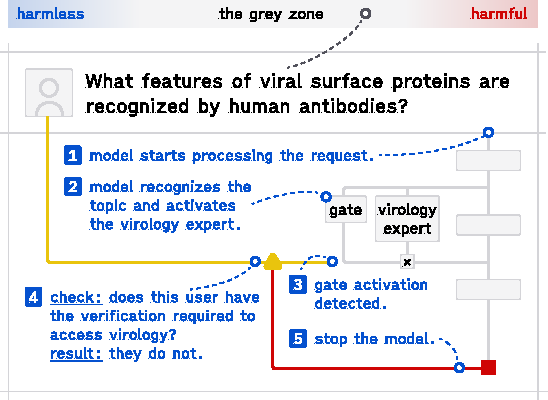
\includegraphics[width=\columnwidth]{assets/main_figure.pdf}}
    \caption{The user is asking a question from the grey zone, that
      is, one that could be either harmless or harmful, depending on
      its real-world context. The schema shows how the question would
      be handled by the system we propose. (1)~The model is trained to
      be helpful and begins to answer the question. (2)~The model
      activates its virology expert module because it contains concepts
      relevant to the question. (3)~The gate activation is observed by
      an external mechanism that immediately (4)~checks if the user has
      the required authorization to access virology knowledge.
      (5)~Since they don't, the model is stopped. If they did, the
    model would be allowed to answer the question.}
    \label{figure:main}
  \end{center}
  \vskip -0.2in
\end{figure}

Safety systems that rely solely on content analysis immediately face
the \emph{dual-use dilemma}. Since the same request can be either
harmless or harmful depending on the context, wherever they draw the
refusal line, they will restrict model utility for legitimate users
while letting slip harmful requests from adversaries. Some safety
systems try to address this by considering real-world context
alongside content. However, they typically infer the context from the
content itself, making it easy for adversaries to fabricate.

In this paper, we argue that informative, hard-to-fabricate
real-world context could be obtained using user-level verifications
such as institutional affiliation, or know-your-customer checks. We
then address the dual-use dilemma with two contributions:
(1) We show how this type of context could be used jointly with
content analysis in a safety system based on access controls
\cite{butler1974}. First, generated content would be classified into
risk categories. Then, a check would be performed to see whether the
user has the verifications required to access the detected
categories. (2) We propose a novel technical approach to risk
category classification that is based on gradient routing
\cite{cloud2024gradientroutingmaskinggradients}. Our proposal avoids
having the capability gap between a model and its monitors that can
make output monitoring methods non-robust
\cite{jin2024jailbreakinglargelanguagemodels}.

Our framework is a first step toward solving the challenge of
``detection and authorization of dual-use capability at inference
time'' that was highlighted by a recent survey of problems in
technical AI governance \cite{reuel2025openproblemstechnicalai} and
also raised by the \citet{NIST_AI_800_1_ipd_2024}.
As such, it has important governance implications, potentially
enabling a more nuanced regulatory approach where access to powerful
AI capabilities is stratified rather than binary, with policies that
differentiate between user types and user contexts rather than
focusing solely on model capabilities. While choosing the appropriate
verification mechanisms and the risk categories remains for future
work --- which should ideally happen jointly with stakeholders from
academia, AI governance, and industry --- our approach offers a
promising direction for addressing the dual-use dilemma.

\section{Current Safety Methods Don't Solve the Dual-Use Dilemma}
\label{section:current-methods}

We evaluate three AI safety approaches to see how sensitive they are
to contextual information, and whether their sources of real-world
context are trustworthy --- that is, hard to manipulate by an adversary.

But first, to illustrate the need for context, consider decomposition
attacks \cite{glukhov2023llmcensorshipmachinelearning,
glukhov2024breachthousandleaksunsafe}: transforming a clearly harmful
query, such as ``How to modify a virus to avoid immune detection?'',
into a series of mundane technical questions, like the ``What
features of viral surface proteins are recognized by human
antibodies?'' from \cref{figure:main}. Here, the attacker exploits
the dual-use dilemma, and the fact that model providers can't refuse
grey zone requests to preserve model utility.

\subsection{Unlearning}

Unlearning methods aim to remove specific knowledge, concepts, or
capabilities from a model after training
\cite{liu2024rethinkingmachineunlearninglarge}. Their goal is to
eliminate the model's ability to generate harmful content while
preserving other capabilities.

Unlearning faces significant technical challenges even for preventing
clearly harmful behaviours. As noted by \citet{cooper2024machineunlearningdoesntthink} and
\citet{barez2025openproblemsmachineunlearning}, capabilities are hard
to define, hard to link to specific data points, and hard to remove
without side effects. Many unlearning approaches mask rather than
truly remove the targeted knowledge
\cite{deeb2025unlearningmethodsremoveinformation}. Moreover, even
nascent robust unlearning methods
\cite{cloud2024gradientroutingmaskinggradients} are not contextual,
and thus don't address the dual-use dilemma without additional assumptions.

\subsection{Safety Training}

Safety training methods modify the model's training process to align
its outputs with human preferences. This category includes safety
pre-training \cite{maini2025safetypretraininggenerationsafe}, RLHF
\cite{christiano2023deepreinforcementlearninghuman}, and safety finetuning.

Unlike unlearning, these methods are contextual. They don't remove
capabilities entirely but train the model to selectively deploy them
based on, among other things, the perceived legitimacy and
harmlessness of the request.

However, the real-world context comes from an untrustworthy source
--- it is entirely (implicitly) inferred from the request's content
which is supplied by the user. This constrains the model's ability to
make truly informed decisions about grey zone requests, making it
susceptible to attacks that fabricate context
\cite{zeng2024johnnypersuadellmsjailbreak} or diminish the model's
context-sensitivity through multi-round escalation
\cite{russinovich2025greatwritearticlethat}.
Thus, despite offering improved contextuality over unlearning,
current safety training methods can't robustly address the dual-use dilemma.

\subsection{Post-Processing}

Post-processing methods apply separate monitoring and filtering
systems to evaluate user inputs and model outputs for harmfulness
\cite{inan2023llamaguardllmbasedinputoutput,
sharma2025constitutionalclassifiersdefendinguniversal} or classify
them into categories \cite{handa2025economictasksperformedai}.

Post-processing methods are contextual, making case-by-case decisions
for each output and thus having the capacity to consider per-output
real-world context.

However, similarly to safety training, the context they implicitly
work with is currently inferred from the request's content and is
thus untrustworthy and vulnerable to similar attacks, as evidenced by
the many jailbreaks that successfully target current production
systems \cite{zhang2025outputconstraintsattacksurface}. Nevertheless,
these methods could be modified to incorporate external contextual
information, potentially serving as a foundation for more
trustworthy, contextual safety mechanisms. We discuss this option in
\cref{section:risk-classification}.

\section{Access Controls as a Feasible Solution}
\label{section:access-controls}

In the previous section, we established that current safety systems
do not address the dual-use dilemma because they either do not
consider the real-world context of the request, or they obtain the
context directly from the request's content, making them vulnerable
to adversarial attacks. In this section, we present an alternative
safety framework based on access controls that directly addresses the
dual-use dilemma, and discuss some of its practical considerations.

\subsection{The Access Control Framework}

Taking note of the problems of current safety methods, we first need
a trustworthy source of real-world context. Drawing inspiration from
other industries, we propose user-level verification mechanisms as a
feasible way to obtain informative context about the user (and by
extension, their requests). These verifications could range from
basic identity confirmation to institutional affiliation to thorough
know-your-customer (KYC) checks \cite{FATF2025}, each granting
different access permissions.

To utilize this user-level context for addressing the dual-use
dilemma, we recommend implementing an access control system: (1)
pre-define multiple risk categories such as advanced virology or
cybersecurity; (2) train classifiers to determine whether a given
model output belongs to these categories (see
\cref{section:risk-classification}); and (3) check whether the user
has the required verifications for generating content in that
category. The verification requirements should be publicly available,
enabling users to obtain necessary credentials ahead of time.

In practice, harmless content would require no verification,
preserving frictionless experience for everyday queries. Grey zone
outputs would require a level of verification calibrated to their
risk assessment. For example, the virology question from
\cref{figure:main} might require the user to be affiliated with a
recognized research facility. Clearly harmful requests would still be
refused outright.

This defensive-by-default approach aims to minimize the attack
surface by aligning with the principle of least privilege
\cite{1451869}. It prevents unauthorized users from executing
decomposition attacks while not reducing model utility for legitimate
users, or even potentially granting advanced users access to more
capabilities, as developers would no longer need to draw arbitrary
refusal lines. The system thus enhances both utility for legitimate
users and overall safety, solving the dual-use dilemma.

\subsection{Practical Considerations}
\label{section:access-controls-future-work}

Many questions about the implementation of the system remain open for
future work.

\textbf{Verification levels} must take into account feasibility,
trustworthiness, user privacy, and the risk assessment of the
different risk categories.
We propose a two-tier verification system as an initial
implementation. Most capabilities require no verification,
maintaining frictionless access for common use cases. Institutional
verification (required only for high-risk domains) consists of
organizational email verification, and affiliation confirmation from
authorized representatives. This verification would be performed by
third parties with existing identity verification infrastructure.

\textbf{Risk categories} must balance granularity with technical
feasibility, reflecting usage patterns, potential harm,
classification reliability, and the friction of their assigned
verification level. Initially, content could fall into two risk
categories. Standard content (requiring no verification) includes
general programming and everyday queries. High-risk content
(requiring institutional verification) includes: advanced
bioengineering, chemical synthesis, and advanced cybersecurity (e.g.,
beyond the most basic textbooks). These categories represent
specialized knowledge with clear misuse potential yet legitimate
research applications.

\textbf{System responses} can vary based on risk category and
classification confidence.
The initial implementation might use a three-phase response system:
(1) For outputs belonging to a risk category with high-confidence,
immediate refusal with a specific explanation of the verification
required; (2) For borderline classifications, continued generation
with enhanced logging and post-processing review; (3) For verified
users, seamless access with background logging for audit purposes.

\subsection{Analysis of Feasibility}

\textbf{False positives} might be a problem, especially in early
implementations of the system, increasing friction for users. This
friction might necessitate external coordination to encourage
adoption across the industry.

\section{Implementing Risk Classification} \label{section:risk-classification}

A core requirement of the verification-based access control system
described in \cref{section:access-controls} is being able to reliably
classify model outputs into risk categories.
This classification needs to address key challenges: accuracy with
minimal false positives, resistance to adversarial attacks, and efficiency.
We examine two approaches to implementing this classification --- one
currently available and one theoretical --- and discuss their trade-offs.

\subsection{Post-Processing}

As discussed in \cref{section:current-methods}, current systems
already rely on post-processing classifiers that analyse outputs
before delivery to users.
These could be adapted for content classification into risk
categories in an access control system.
For example, a classifier could be trained to identify moderately
advanced virology topics and, if detected, could trigger verification
of user permissions before delivering the output.

The key advantage of post-processing systems is modularity, as they
can be developed and updated independently of the generation models
they oversee.
However, they face a trade-off between usability (latency) and safety
\cite{kumar2025freelunchguardrails}: prioritizing low latency can
create a capability gap between generators and monitors that
sophisticated language models can exploit
\cite{jin2024jailbreakinglargelanguagemodels}.
Despite this limitation, recent post-processing methods show
acceptable efficiency and resilience toward jailbreaks
\cite{sharma2025constitutionalclassifiersdefendinguniversal} and
could provide a practical initial implementation path for
output-based access control.

\subsection{Gradient Routing} \label{section:gradient-routing}

To address the capability gap problem in post-processing methods, we
detail how gradient routing \cite{cloud2024gradientroutingmaskinggradients}
could be adapted to classify model outputs into risk categories.
Our adaptation represents a theoretical direction for integrating
risk category detection directly into model architecture.
This approach can be combined with post-processing methods and offers
different trade-offs.

We propose augmenting models with small expert modules controlled by
learned gates, as shown in \cref{figure:main}.
During model training, assuming we have examples from the relevant
risk categories (e.g., advanced virology), the expert module would be
made to receive gradients exclusively from these examples.
Simultaneously, the module's gate would be trained to activate the
module on these examples using an auxiliary loss function.
We hypothesize this would lead to the module obtaining specialist
knowledge from the risk domain, and to the model learning to activate
the module whenever this knowledge is needed.

\Cref{figure:main} illustrates this in the context of the wider
access control system: when a user requests information about viral
surface proteins, the model correctly recognizes the domain and
activates the virology gate, engaging the expert but also triggering
the verification system. If the user lacks appropriate credentials,
the system takes the appropriate response --- here, halting the generation.

This approach eliminates the efficiency-capability
trade-off inherent in post-processing methods: the risk category
classifier is embedded within the larger model, so there is no
capability gap, and because the gated module is small and integrated
into the model's forward pass, it is computationally efficient with
minimal impact on latency.

Even more crucially, during standard training, the model is naturally
incentivized to identify risk category information in inputs and
surface this in its representation space, as this is directly linked
to enabling the appropriate specialized module at appropriate times.
This approach differs fundamentally from post hoc methods like
probing or sparse autoencoders
\cite{cunningham2023sparseautoencodershighlyinterpretable}, which
cannot guarantee the model actually operates with the concepts they
attempt to identify.
Additionally, it resolves the adversarial dynamic (model vs.
monitors, helpful vs. harmless) common in AI safety by aligning
training incentives with safety objectives.

Several technical challenges remain. While gradient routing has shown
promise in creating specialized modules in smaller models, its
effectiveness in larger language models, particularly with the
gated-expert architecture, requires empirical validation. Other key
challenges include preventing false positives and false negatives,
though regularization techniques and adjusted detection thresholds,
respectively, could mitigate these issues. Our approach also requires
identifying risk categories during initial training, prompting
research into adaptation of gradient routing for fine-tuning
scenarios. Despite these challenges, the approach offers promising
theoretical properties that warrant experimental investigation.

\section{Limitations and Tradeoffs}

Our framework presents inevitable trade-offs --- privacy concerns,
access inequities, and increased friction through false positives ---
but these can be addressed through improved verification mechanisms
and continuously improving classification systems. Future work needs
to determine appropriate verification levels and risk categories,
develop accurate classifiers with low false positive rates, and align
with emerging AI regulations through stakeholder engagement. We
discuss some of these challenges in
\cref{section:access-controls-future-work} and at the end of
\cref{section:gradient-routing}.

\section{Conclusion}

We argued that safety systems that do not utilize contextual
information face a lose-lose \emph{dual-use dilemma}: they will
restrict model utility for some legitimate users while still allowing
some adversaries to use the model for ill. To address this problem,
we introduced a new access control framework that limits access to
outputs from certain risk categories only to users with relevant
verifications (which serve as proxies for trustworthy real-world
context). We also proposed a novel technical solution for classifying
outputs into risk categories based on gradient routing that has the
potential to resolve the efficiency-robustness trade-off of
post-processing methods.

Beyond addressing specific technical challenges, our framework
represents a promising governance shift from working with model-level
abstractions and binary capability restrictions toward more granular
user-level access controls. This offers a practical pathway for
regulating increasingly powerful AI systems through stratified access
rather than blanket capability limitations.

\section{Acknowledgements}

We thank Dennis Akar, Jakub Kryś, and Kola Ayonrinde for their feedback on a draft of this paper. We thank Joseph Miller, Alex Cloud, Alex Turner, and Jacob Goldman-Wetzler for discussions on gradient routing.

\bibliography{references}
\bibliographystyle{packages/icml2025}

%%%%%%%%%%%%%%%%%%%%%%%%%%%%%%%%%%%%%%%%%%%%%%%%%%%%%%%%%%%%%%%%%%%%%%%%%%%%%%%
%%%%%%%%%%%%%%%%%%%%%%%%%%%%%%%%%%%%%%%%%%%%%%%%%%%%%%%%%%%%%%%%%%%%%%%%%%%%%%%
% APPENDIX
%%%%%%%%%%%%%%%%%%%%%%%%%%%%%%%%%%%%%%%%%%%%%%%%%%%%%%%%%%%%%%%%%%%%%%%%%%%%%%%
%%%%%%%%%%%%%%%%%%%%%%%%%%%%%%%%%%%%%%%%%%%%%%%%%%%%%%%%%%%%%%%%%%%%%%%%%%%%%%%
\newpage
\appendix
\onecolumn

\end{document}

% This document was modified from the file originally made available by
% Pat Langley and Andrea Danyluk for ICML-2K. This version was created
% by Iain Murray in 2018, and modified by Alexandre Bouchard in
% 2019 and 2021 and by Csaba Szepesvari, Gang Niu and Sivan Sabato in 2022.
% Modified again in 2023 and 2024 by Sivan Sabato and Jonathan Scarlett.
% Previous contributors include Dan Roy, Lise Getoor and Tobias
% Scheffer, which was slightly modified from the 2010 version by
% Thorsten Joachims & Johannes Fuernkranz, slightly modified from the
% 2009 version by Kiri Wagstaff and Sam Roweis's 2008 version, which is
% slightly modified from Prasad Tadepalli's 2007 version which is a
% lightly changed version of the previous year's version by Andrew
% Moore, which was in turn edited from those of Kristian Kersting and
% Codrina Lauth. Alex Smola contributed to the algorithmic style files.
